\documentclass[a4paper, fontsize=11pt]{scrartcl}
\usepackage{enumitem}
\usepackage{amssymb}
\usepackage{tikz}
\usetikzlibrary{shapes, arrows.meta, positioning, calc, fit, shapes.geometric, shapes.multipart, shapes.arrows, decorations.pathreplacing}



% Setup document
% Import Eidesstattliche Erklärung
\usepackage{pdfpages}
% Import graphics and wrap them
\usepackage{graphicx}
\usepackage{wrapfig}
\usepackage{float}

% Localization
\usepackage[utf8]{inputenc}
\usepackage[T1]{fontenc}
\usepackage[ngerman]{babel}

% Clickable table of contents
\usepackage{hyperref}
\usepackage[ngerman]{cleveref}

% Page formatting
\usepackage[automark]{scrlayer-scrpage}
\usepackage{typearea}
\usepackage{microtype}

% Better tables
\usepackage{tabularray}
\usepackage{booktabs}

% Develop Packages
\usepackage{blindtext}
% Variables
\newcommand{\vorname}{Lukas}
\newcommand{\nachname}{Szimtenings}
\newcommand{\matr}{Matr.-Nr.\ 3217694}
\newcommand{\uni}{FH Aachen}
\newcommand{\studiengang}{Angewandte Mathematik und Informatik}
\newcommand{\modul}{5. Semester 952006 (Aachen)}
\newcommand{\erstpruefer}{Alexander Voß}
\newcommand{\zweitpruefer}{Raphael Majeed}
\newcommand{\subtitel}{ Verteilte Ausführung von in konjunktiver Normalform spezifizierten Machbarkeitsabfragen in medizinischen Datenintegrationszentren }
\newcommand{\titel}{- Seminararbeit -}
\newcommand{\location}{Aachen}
\newcommand{\abteilung}{Abteilung: Research Infrastructure}
\newcommand{\abteilungabkuerzung}{RI}

%images
\newcommand{\uklogo}{
    
\includegraphics[scale=0.5]{res/logo-uniklinik-rwth-aachen}
    
\includegraphics[scale=0.6]{res/imi_sublogo}
}

\newcommand{\ukimilogo}{
\includegraphics[scale=0.16]{res/imilogo}}
% command for wrapfigure -> more than one figure per paragraph
\newcommand*{\invisiblepar}{{\setlength{\parfillskip}{0pt}\par}\vskip-\parskip\noindent\ignorespaces}
% Metadata
\title{\titel}
\author{\vorname{} \nachname}
\date{\today{}, \location}

% Pagestructure
\clearpairofpagestyles
%footer
\ifoot[]{\ukimilogo}
\cfoot[]{\abteilungabkuerzung}
\ofoot[]{\pagemark}
%header
\ihead[]{\vorname\ \nachname}
\chead[]{\titel}
\ohead[]{\matr}
%Seperator
\setheadsepline[\textwidth]{1pt}
\setfootsepline[\textwidth]{1pt}
\addbibresource{Seminararbeit.bib}


\begin{document}
%% Prefix %%
% Titelblatt
\begin{titlepage}
    \centering
    {\scshape\LARGE \uni{} \par \studiengang{} \par \modul{} \par}
    \vspace{1cm}
    {\scshape\Large \titel{} \par}
    \vspace{1.5cm}
    {\bfseries \huge \subtitel{} \par}
    \vspace{2cm}
    {\Large \vorname{} \nachname{} \par \matr{} \par}
    \vfill
    \begin{center}
        \itclogo{}
        \par
        \abteilung{}
    \end{center}

    \par\vfill
    \parbox{4cm}{\hrule \strut{} \centering \footnotesize \vorname{} \nachname{} \par \textit{Autor}}
    \hfill
    \parbox{5cm}{\hrule \strut{} \centering \footnotesize \erstpruefer{} \par \textit{Erstprüfer}}
    \hfill
    \parbox{4cm}{\hrule \strut{} \centering \footnotesize \zweitpruefer{} \par \textit{Zweitprüfer}}
    \vfill
    {\large \location{} \today \par}
\end{titlepage}
% Einbinden der Eidesstattlichen Erklärung
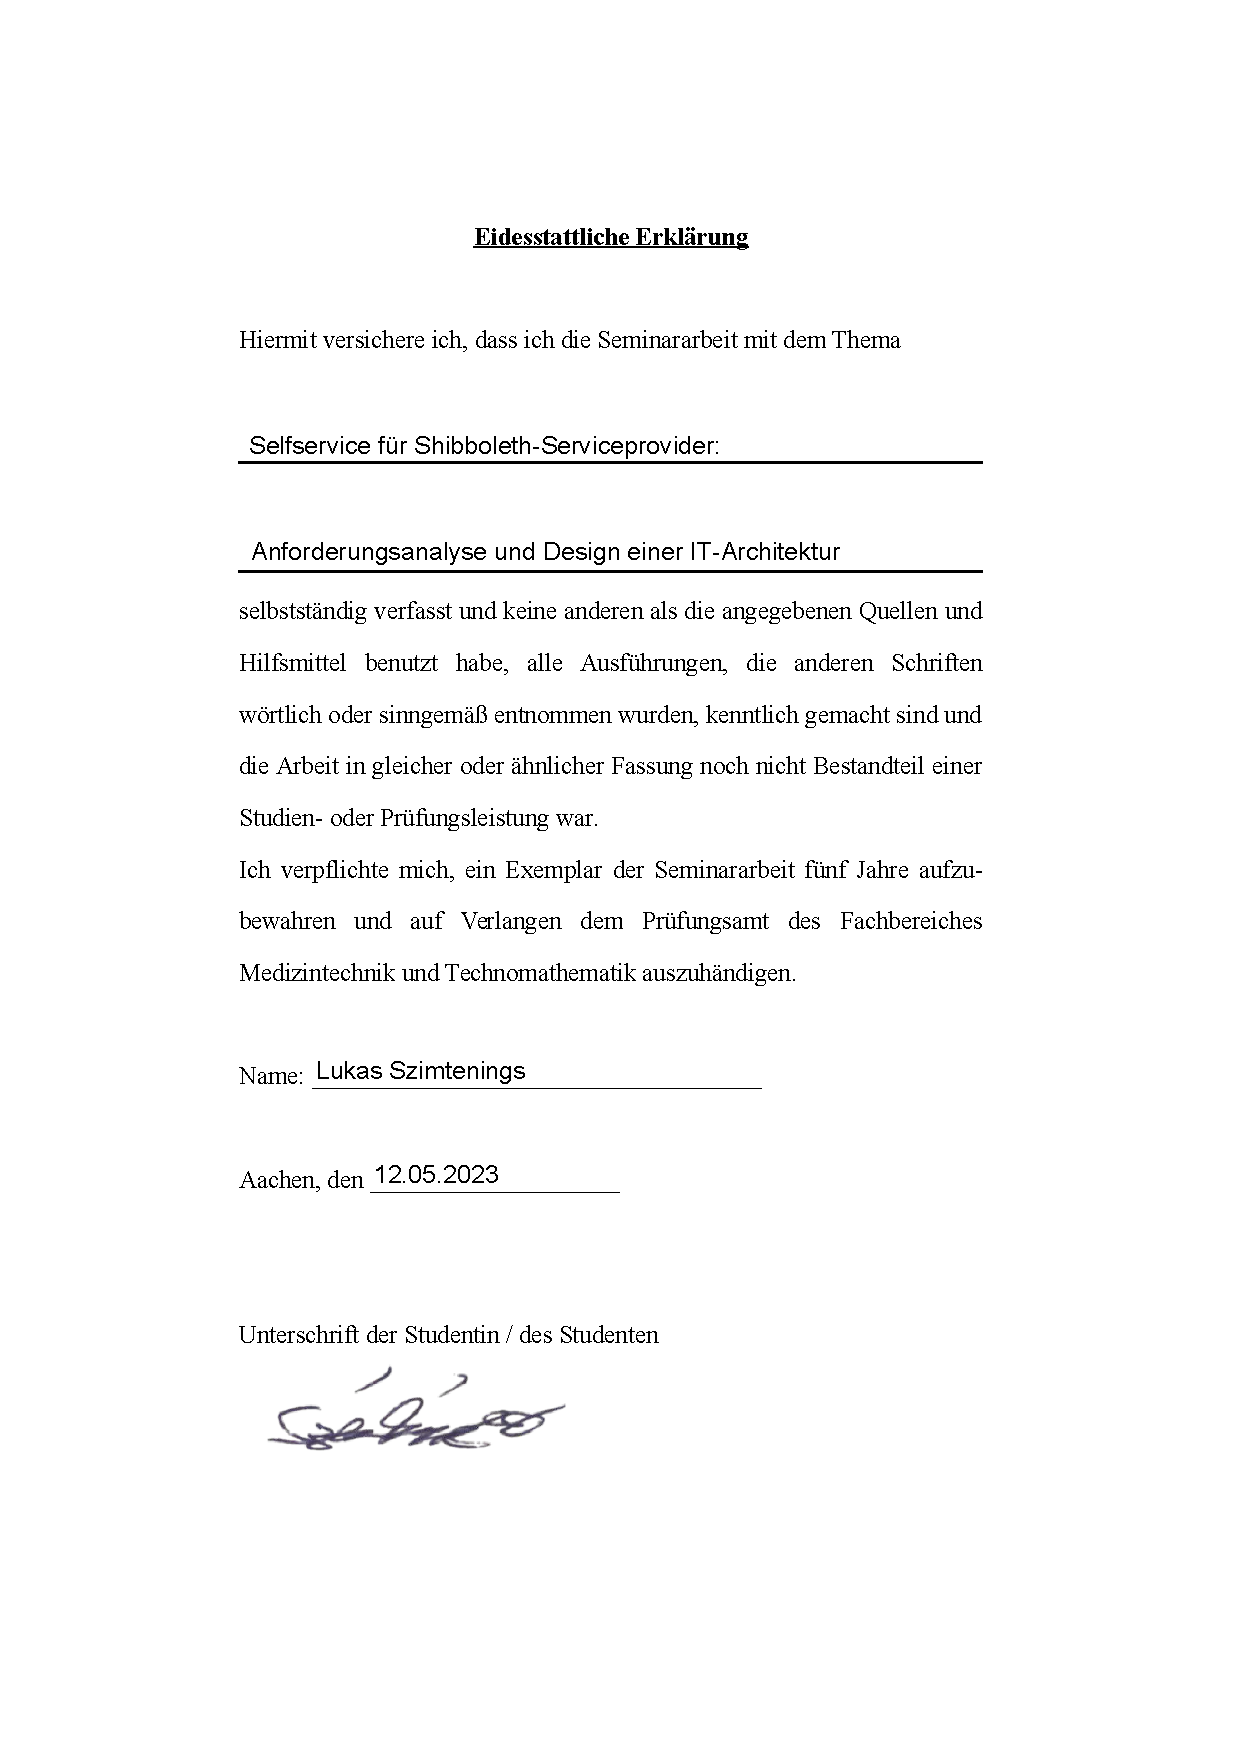
\includepdf{res/EidesstattlicheErklaerung.pdf}
\tableofcontents
\newpage

%% Hauptteil %%
% Seitenzahlen beginnen ab hier
\pagenumbering{arabic}

\section{Einführung}\label{sec:einfuehrung}
Die zunehmende Digitalisierung in Unternehmen führt dazu, dass Prozesse immer mehr automatisiert werden müssen, um wettbewerbsfähig zu bleiben.
Dabei stellt insbesondere die Verwaltung von Zugriffsberechtigungen eine Herausforderung dar, da diese oft sehr komplex und zeitaufwändig ist.
Eine Möglichkeit Zugriffsberechtigungen auf Systeme einer ganzen Organisation und darüber hinweg föderiert zu verwalten ist die Nutzung eines Single Sign-On (SSO) Systems.
Die RWTH Aachen verwendet bereits ein solches System, musste jedoch feststellen, dass durch die Verwaltung von Serviceprovidern ein nicht geringer administrativer Aufwand anfällt.
Zur Entwicklung eines Self-Service Systems muss daher zunächst die Verwaltung von Serviceprovidern auf der Prozessebene analysiert werden.

\subsection{Problemstellung}\label{subsec:problemstellung}
Ein SSO System besteht in aller Regel aus mindestens zwei Komponenten, zum einen dem Identity Provider (IDP) welcher konzeptionell Nutzer authentifiziert und autorisiert, und dem Service Provider (SP) welcher auf Basis der Informationen vom IDP über den Nutzer Zugriff auf seine Ressourcen gewährt.
Das von der RWTH betriebene Shibboleth ist ein solches System, welches vielseitigen Einsatz an der RWTH und übergeordneten Organisationen findet.
Da aus Sicherheitsgründen nicht jeder SP Zugriff auf das SSO System erhalten soll, muss die Verwaltung von SPs zentral in der Hand des IDPs liegen. 
Dies führt jedoch zu einem hohen Verwaltungsaufwand, da die Anzahl der SPs stetig wächst und die Verwaltung der Zugriffsberechtigungen für jeden SP händisch in der IDP Konfiguration erfolgt.
Da die Konfigurationsdatei eine Sicherheitsrelevante Resource darstellt, ist die Anzahl der Personen die diese bearbeiten dürfen begrenzt.

\subsection{Metadaten}
Bei der in der Problemstellung erwähnten Verwaltung von SPs fallen verschiedene sogenannte Metadaten an, die für die Kommunikation und das Verständnis zwischen den beteiligten Systemen wichtig sind. Die wichtigsten Metadaten sind:

\begin{itemize}
    \item \textbf{Entity-IDs:} Eindeutige Bezeichner für die beteiligten Systeme, z. B. für Identity Provider und Service Provider. Die Entity-IDs werden in den Metadaten verwendet, um die Kommunikation zwischen den Systemen zu ermöglichen.
    \item \textbf{Endpunkte (Endpoints):} URLs, über die SAML-Anfragen und -Antworten ausgetauscht werden. Dazu gehören die Single Sign-On Service (SSOS) und Single Logout Service (SLOS) Endpunkte des IdPs sowie die Assertion Consumer Service (ACS) und Single Logout Service (SLOS) Endpunkte des SPs.
    \item \textbf{Zertifikate:} X.509-Zertifikate, die für die Signierung und Verschlüsselung von SAML-Nachrichten verwendet werden. Die öffentlichen Schlüssel aus diesen Zertifikaten werden in den Metadaten veröffentlicht, damit die Kommunikation zwischen IdP und SP sicher erfolgen kann.
    \item \textbf{Attribute:} Informationen über den Benutzer, die vom IdP an den SP weitergegeben werden. Die Nutzerattribute (z. B. E-Mail-Adresse, Benutzername, Abteilung) welche an den jeweiligen SP bei einem login weitergegeben werden, werden in den Metadaten definiert, und müssen daher auch verwaltet werden.
    \item \textbf{Bindings und Profile:} SAML-Bindings legen fest, wie SAML-Nachrichten über HTTP transportiert werden (z. B. POST, Redirect oder SOAP). SAML-Profile definieren den Ablauf und die Struktur von SAML-Nachrichten für bestimmte Anwendungsfälle (z. B. Web Browser SSO oder Single Logout). Diese Informationen sind ebenfalls in den Metadaten enthalten.
\end{itemize}

Die Verwaltung der Metadaten erfolgt in der Regel über einen zentralen Metadatenspeicher, wie z. B. einen Metadatenaggregator oder einen Metadatendienst. 
Die beteiligten Systeme (IdPs und SPs) stellen ihre eigenen Metadaten bereit und beziehen die Metadaten der anderen Systeme aus dem zentralen Speicher. 
Dadurch wird eine konsistente und vertrauenswürdige Informationsbasis für die Kommunikation und das Verständnis zwischen den Systemen sichergestellt.\\
Die Metadaten werden in der Regel in einem XML-Format ausgetauscht und von Administratoren in die zugehörigen Konfigurationsdateien eingetragen. 
Sicherheitsmechanismen wie Signierung der Metadaten und regelmäßige Überprüfungen der Zertifikate sind notwendig, um die Integrität und Vertraulichkeit der Metadaten zu gewährleisten.

\subsection{Zielsetzung}\label{subsec:zielsetzung}
Ziel dieser Seminararbeit ist es daher, die Verwaltung von SPs auf der Prozessebene zu analysieren und zu modelieren.
In einer Anforderungsanalyse soll dann erarbeitet werden, welche Anforderungen ein Self-Service System erfüllen muss um möglichst viele Teilprozesse an SP Betreiber auszulagern.
\subsection{Abgrenzung}\label{subsec:abgrenzung}
Nicht Ziel dieser Arbeit ist es, ein Systementwurf oder gar Code zu erstellen.
Es soll lediglich eine Analyse der Prozesse erfolgen, und auf Basis dieser eine Anforderungsanalyse durchgeführt werden.


\section{Grundlagen}\label{sec:grundlagen}
   \subsection{Prozessanalyse}\label{subsec:prozessanalyse}
   \subsection{Anforderungsanalyse}\label{subsec:anforderungsanalyse}

\section{Methodik}\label{sec:methodik}
Hier erkläre ich warum ich welche der oben genannten Methoden gewählt habe und wie ich sie im Detail angewandt habe
\subsection{Prozessmodelierung}\label{subsec:prozessmodelierung-methodik}
\subsection{Auswahl der Gesprächspartner}\label{subsubsec:auswahl-gespraechspartner}
Die Festlegung der Stakeholder-Gruppen für die Befragung zum Zwecke der Prozessmodellierung erfolgte durch eine Dokumentenanalyse der öffentlich zugänglichen Shibboleth-Dokumentation. 
Die Dokumentenanalyse ist eine manuelle Technik zur Business Process Discovery, die im Abschnitt~\ref{subsubsec:discovery-manuelle-techniken} kurz vorgestellt wird. 

\subsubsection{Identity Provider (IDP)}
Die zentrale Rolle der IDPs bei der Verwaltung von Metadaten und der Bereitstellung von Zugriffskontrollen wurde durch die Dokumentenanalyse der Shibboleth-Dokumentation ermittelt. 
Aufgrund ihrer Verantwortung für die Eingabe und Aktualisierung von Metadaten wurde die Stakeholder-Gruppe der IDP-Administratoren ausgewählt.

\subsubsection{Service Provider (SP)}
Die Dokumentenanalyse der Shibboleth-Dokumentation verdeutlichte desweiteren die Verantwortung der SPs für die Bereitstellung von Diensten und die Umsetzung von Zugriffsrichtlinien, die auf den vom IDP gelieferten claims basieren.
Um den Reibungslosen Ablauf der Kommunikation mit dem IDP sicher zu stellen, müssen die SPs den IDP mit ihren Metadaten versorgen, und diese bei Änderungen aktualisieren.
Die Stakeholder-Gruppe der SP-Administratoren wurde daher ausgewählt, um ihre Erfahrungen und Anforderungen hinsichtlich der Metadatenverwaltung zu untersuchen.

\subsection{Entwurf des Fragenkatalogs}\label{subsubsec:entwurf-fragenkatalog}

In diesem Abschnitt stellen wir Fragen für die verschiedenen Stakeholder-Gruppen auf: Projektverantwortliche, Administratoren der IDP, die für die Eingabe von Metadaten verantwortlich sind, und Serviceanbieter-Administratoren. 
Diese Fragen zielen darauf ab, detaillierte Informationen zur Verwaltung von Metadaten zu sammeln und ihre Relevanz für das Prozessmodellierung zu untersuchen.
Die Erstellung des Fragenkatalogs ist auf Grundlage der in Kapitel~\ref{subsec:interviews-grundlagen} vorgestellten Kriterien erfolgt.

\subsubsection{Administratoren des IDP}

\textbf{Welche Arten von Metadaten verwalten sie derzeit?}\\
Da unterschiedliche Inhalte auf verschiedene Art und Weise verwaltet werden könnten, woraus unterschiedliche Prozesse entspringen könnten, versucht diese Frage die verschiedenen Metadaten zu identifizieren.\\\\
\textbf{Wie werden neue Serviceprovider angelegt und verifiziert?}\\
Ziel der Frage ist es, offen zu legen interessierte Serviceprovider einen Zugang zum Identityprovider erhalten. Besonderes Augenmerk ist dabei zu legen auf die Prüfung von Authentifizierung und Authorisierung der Interessenten\\\\
\textbf{Wie werden Metadatenänderungen kommuniziert und wie wird sichergestellt, dass alle relevanten Parteien informiert werden?}\\
Der Teilprozess der Kommunikation zwischen Serviceprovider und Identityprovider soll durch diese Frage identifiziert werden. Im Fokus steht hier unter anderem der durch Kommunikation entstehende Mehraufwand.\\\\
\textbf{Wie werden Metadatenänderungen validiert und wie wird sichergestellt, dass bei der Eintragung keine Fehler auftreten?}\\
Die Korektheit der eingetragenen Änderungen ist ein wichtiges Qualitätsmerkmal des Prozesses, die Frage zielt daher darauf ab den Teilprozess zu identifizieren welcher die Richtigkeit und Vollständigkeit gewährleistet\\\\
\textbf{Gibt es Schwierigkeiten bei der Verwaltung von Metadaten, die aufgrund des aktuellen Prozesses auftreten}?\\
 Die Identifikation von wahrgenommenen Schwachstellen in dem Prozess durch involvierte Akteure liefert wichtige Informationen für die folgende Prozessanalyse\\\\
\textbf{Wie werden Metadatenänderungen in der IDP-Konfiguration vorgenommen?}\\
Die Änderung der Metadaten ist der Kern des Prozesses, und muss somit modelliert werden. Des weiteren kann diese Frage die verwendete Technologiebasis offen legen und damit wichtige Vorarbeit für die Anforderungsanalyse liefern.\\\\
\textbf{Wie viel Zeit wird derzeit für die Verwaltung von Metadaten aufgewendet?}\\
Ziel der Frage ist es, die Auswirkungen des Prozesses auf die Arbeitsbelastung der involvierten Akteure zu erfassen. Diese Information wird wichtig sobald die Priorisierung einzelner Teilprozesse für einen Zukünftigen Selfservice im Rahmen der Anforderungsanalyse vorgenommen werden muss.\\\\

\subsubsection{Serviceprovider-Administratoren}
\textbf{Wie gehen sie vor wenn sie Änderungen an ihrem Serviceprovider kommunizieren wollen}\\
Ziel der Frage ist es, einen Vergleich zu den Aussagen des IDP zu schaffen.\\\\
\textbf{Gibt es Schwierigkeiten bei der Verwaltung von Metadaten, die aufgrund des aktuellen Prozesses auftreten}?\\
Die Identifikation von wahrgenommenen Schwachstellen in dem Prozess durch involvierte Akteure liefert wichtige Informationen für die folgende Prozessanalyse\\\\
\textbf{Wie würden sie die Kommunikation mit der IDM-Gruppe beschreiben?}\\
Die Frage zielt darauf ab, Qualitative Probleme in der Kommunikation offen zu legen.\\\\


Diese Fragen behandeln die verschiedenen Aspekte der Metadatenverwaltung und deren Relevanz für das Prozessmodellierung aus der Perspektive der verschiedenen Stakeholder-Gruppen.

\section{Prozessbeschreibung}

Diese Prozessbeschreibung basiert auf einem Interview mit einem Mitarbeiter des Identity Management Teams (IDM) einer Organisation, die sich mit der Verwaltung von Metadaten für Serviceprovider (SP) beschäftigt.
Der Prozess umfasst die Verwaltung von externen und internen Datenquellen, die Kommunikation mit den Service Providern und die Pflege von Metadaten in einem Git-Repository.

\subsection{Ziele und Anforderungen des Prozesses}

Das Hauptziel des Prozesses ist die effektive Verwaltung von Metadaten für Serviceprovider. Dazu gehören:

\begin{itemize}
  \item Die Sammlung und Dokumentation von Informationen zu den Service Providern
  \item Die Prüfung, Aktualisierung und Validierung von Metadaten
  \item Die Kommunikation von Änderungen an relevanten Parteien
  \item Die Sicherstellung der korrekten Konfiguration der Identity Provider (IDP) Server
\end{itemize}

\subsection{Prozesse}

\subsubsection{Neuen Provider eintragen}

\begin{enumerate}
  \item Der SP-Betreiber erstellt beim ITC Servicedesk ein Ticket per E-Mail.
  \item Das Ticket geht an die IDM-Gruppe, die das Ticket auf Informationen prüft.
  \item Die IDM-Gruppe erstellt ein Request-for-Change (RFC)-Dokument (PDF) zur Sammlung und Dokumentation der Informationen.
  \item Das RFC-Dokument wird an den SP gesendet, um evtl.\ fehlende Informationen zu ergänzen und den RFC zu validieren.
  \item Die IDM-Gruppe prüft das RFC-Dokument auf Vollständigkeit und Korrektheit der Informationen.
  \item Bei Fehlern, Rückfragen oder Anpassungen wird wieder mit dem SP kommuniziert.
  \item Während das RFC noch geprüft wird, erhält der SP Zugriff zum Testsystem.
  \item Die IDM-Gruppe prüft den XML-Metadatensatz der aus dem RFC hervorgeht mit einem linter auf Syntaxfehler.
  \item Die IDM-Gruppe fügt den XML-Metadatensatz in das Git-Repository ein
  \item Eine zweite Datei mit Attributfiltern wird aus den angeforderten Attributen im RFC manuell erstellt und in einem anderen Git-Repository gespeichert.
\end{enumerate}

\subsubsection{Bestehende Provider anpassen}

\begin{enumerate}
  \item Der SP-Betreiber identifiziert die Notwendigkeit, die Metadaten eines bestehenden SP zu aktualisieren.
  \item Der SP-Betreiber sendet die aktualisierten Informationen an die IDM-Gruppe, die diese überprüft.
  \item Bei Fehlern, Rückfragen oder Anpassungen wird wieder mit dem SP kommuniziert.
  \item Die IDM-Gruppe verwendet einen XML-Linter, um die XML-Metadaten auf Syntaxfehler zu prüfen.
  \item Die IDM-Gruppe aktualisiert den XML-Metadatensatz und die Attributfilter-Datei in den Git-Repositories entsprechend den aktualisierten Informationen.
  \item Die IDM-Gruppe prüft manuell, ob das Login bei dem Serviceprovider funktioniert.
\end{enumerate}

\subsubsection{Metadatenänderungen in der IDP-Konfiguration vornehmen}

\begin{enumerate}
  \item Die XML-Metadaten in den Git-Repositories werden regelmäßig auf Änderungen überprüft.
  \item Die XML-Dokumente werden automatisch zusammengeführt.
  \item Der Merge wird auf die IDP Server hochgeladen.
\end{enumerate}

\subsection{Kommunikation}
Die Kommunikation im Prozess erfolgt über verschiedene Kanäle:

\begin{itemize}
  \item E-Mail: Hauptkommunikationsmittel für den Austausch von Informationen und Dokumenten
  \item Ticketsystem: Zur initialen Kontaktaufnahme zwischen IDM-Gruppe und SP-Betreiber
\end{itemize}

\subsection{Zeitlicher Aufwand}

Der gesamte zeitliche Aufwand für den Prozess der Metadatenverwaltung kann je nach Komplexität des Falls und der Anzahl der Rückfragen und Diskussionen mit den Serviceprovider Betreibern variieren. 
In der Regel dauert der gesamte Prozess zwischen 3 und 5 Tagen, kann allerdings auch bei Entwicklerwechsel bis zu einem Monat dauern

Von dieser Gesamtdauer entfällt ein erheblicher Teil auf das Abwarten von Rückmeldungen der Serviceprovider Betreiber.
Die effektive Arbeitszeit, die für die Verwaltung der Metadaten benötigt wird, beträgt minimal 4 Arbeitsstunden, und lässt sich dabei in drei Hauptkomponenten unterteilen:

\paragraph{Kommunikation:}
Die Kommunikation zwischen Serviceprovider Betreibern und IDM Gruppe bei Rückfragen zu Attributen ist ein großer Teil des Prozesses.
Die Dauer dieser Kommunikation hängt unter anderem von der Anzahl der offenen Fragen, der Reaktionsgeschwindigkeit der SP-Anbieter, der von den SP-Anbietern geleisteten Vorarbeit und den angefragten Attributen ab. 
Der Zeitaufwand kann daher stark variieren, stellt jedoch in aller Regel einen großen Teil der effektiven Arbeitszeit dar.
\paragraph{Dokumentation}
Im trivialsten Fall fallen für die Dokumentation in Form des RFC 1-2 Stunden an, dies hängt aber wieder von der Komplexität des Falls ab. 
\paragraph{Eintragen, Anpassen und Validieren von Anbindungen:}
Der verbleibende Teil der effektiven Arbeitszeit wird für das eigentliche Eintragen und Anpassen der Anbindungen aufgewendet.
Dies beinhaltet das erstellen des Attributfilters, das einholen der Metadaten von dem SP und das Deployment über die Git-Repositories.
Der Zeitaufwand für diese Aktivitäten kann ebenfalls variieren, allerdings nicht so sehr wie die für die Kommunikation aufgewendete Zeit.


Zusammenfassend kann der Prozess der Metadatenverwaltung in Bezug auf den zeitlichen Aufwand in effektive Arbeitszeit und Wartezeit auf Daten oder Rückmeldungen unterteilt werden. 
Die effektive Arbeitszeit wird hauptsächlich für Kommunikation, Dokumentation und Verwaltungsaufgaben aufgewendet.
\subsection{Modell}
Die Abbildung~\ref{fig:service-provider-erstellung} modelliert den Prozess zur Eintragung eines neuen Service Providers.
% Importiere res/Service Provider Erstellung.png
\begin{figure}[H]
  \centering
  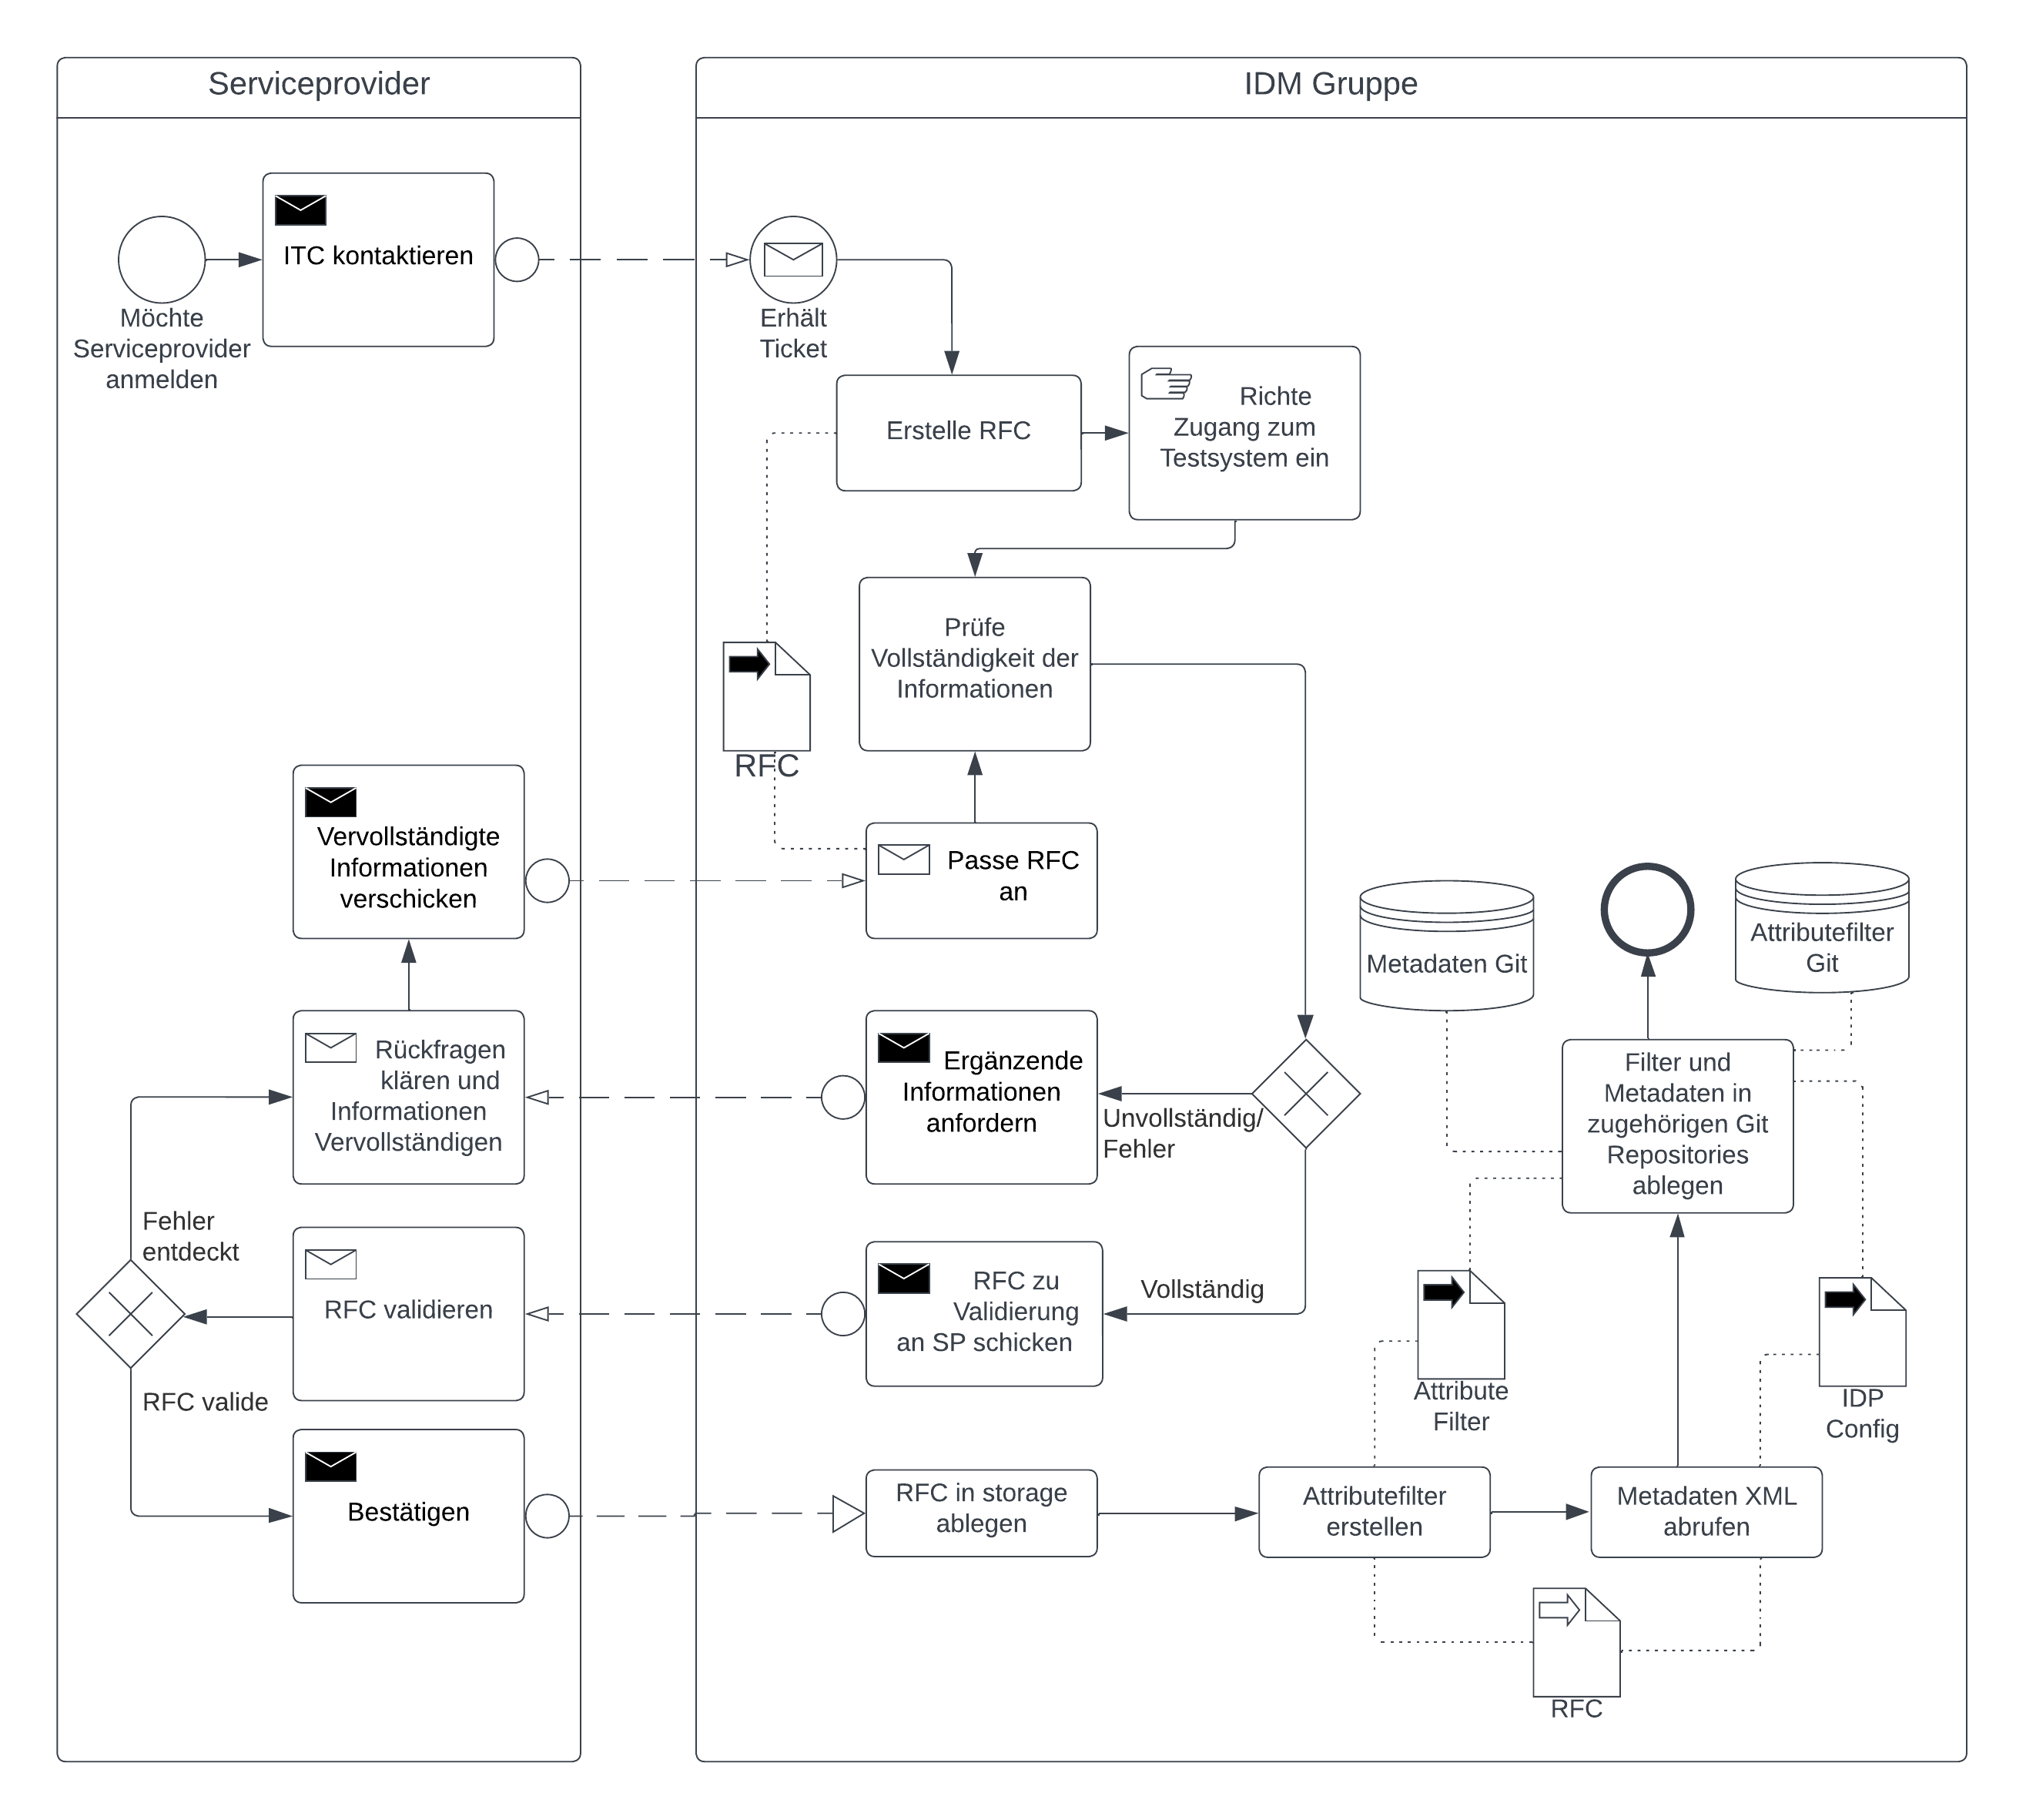
\includegraphics[width=0.8\textwidth]{res/Service Provider Erstellung.png}
  \caption{Prozess zur Eintragung eines neuen Service Providers}\label{fig:service-provider-erstellung}
\end{figure}

Die Abbildung~\ref{fig:service-provider-anpassung} modelliert den Prozess zur Anpassung eines bestehenden Service Providers. Es lässt sich feststellen, dass diese sich nur geringfügig von dem Prozess zur Eintragung eines neuen Service Providers unterscheidet.
% Importiere res/Service Provider Anpassung.png
\begin{figure}[H]
  \centering
  \includegraphics[width=0.8\textwidth]{res/Service Provider Anpassung.png}
  \caption{Prozess zur Anpassung eines bestehenden Service Providers}\label{fig:service-provider-anpassung}
\end{figure}

\section{Ergebnisse und Diskussion}\label{sec:results}
\subsection{Prozessanalyse}\label{subsec:prozessanalyse-results}
\subsubsection{Ergebnisse}\label{subsubsec:prozessanalyse-results}
Ergebnisse bestehend aus zunächst den Fragen und Antworten, und dann dem daraus resultierenden Modell des Prozesses
\subsubsection{Diskussion}\label{subsubsec:prozessanalyse-discussion}
Diskussion der Ergebnisse, eventueller Schwächen im Prozess und Verbesserungsvorschläge
\subsection{Anforderungsanalyse}\label{subsec:anforderungsanalyse-results}
Auflistung der erarbeiteten Anforderungen eingeteilt in funktionale und nicht funktionale Anforderungen
\subsubsection{Funktionale Anforderungen}\label{subsubsec:functional-requirements}
\subsubsection{Nicht-funktionale Anforderungen}\label{subsubsec:non-functional-requirements}
\subsubsection{Diskussion}\label{subsubsec:anforderungsanalyse-discussion}

\section{Zusammenfassung und Ausblick}\label{sec:summary}
\subsection{Zusammenfassung}\label{subsec:summary}
\subsection{Ausblick}\label{subsec:outlook}

%% Suffix %%
\newpage

% Bibliographie
\pagenumbering{Roman}
\printbibliography{}
% Abbildungsverzeichnis
\listoffigures
\end{document}